%%%%%%%%%%%%%%%%%%%%%%%%%%%%%%%%%%%%%%%%%%%%%%%%%%%%%%%%%%%%%%%%%%%%%%
% How to use writeLaTeX: 
%
% You edit the source code here on the left, and the preview on the
% right shows you the result within a few seconds.
%
% Bookmark this page and share the URL with your co-authors. They can
% edit at the same time!
%
% You can upload figures, bibliographies, custom classes and
% styles using the files menu.
%
%%%%%%%%%%%%%%%%%%%%%%%%%%%%%%%%%%%%%%%%%%%%%%%%%%%%%%%%%%%%%%%%%%%%%%

\documentclass[12pt]{article}

\usepackage{sbc-template}
\usepackage{graphicx,url}
\usepackage[utf8]{inputenc}  
\usepackage{amsmath}
\usepackage{tabularx}
\usepackage{amssymb}
\usepackage{multirow}
\usepackage{booktabs}
\usepackage{siunitx}




\sloppy

\title{Learning with Few: A Comparative Study of Multilingual Text Anomaly Detection}

\author{Fabio Masaracchia Maia\inst{1}, Anna Helena Reali Costa\inst{1}}

\address{Escola Politécnica, Universidade de São Paulo, São Paulo, Brazil\\
 \email{fabio.masaracchia@gmail.com, anna.reali@usp.br}
}

% \author{Double-blind\inst{1}}
% \address{double-blind\\
%  % \email{double-blind}
% }
\begin{document} 

\maketitle

\begin{abstract}
Detecting anomalies in textual data is a critical task in domains such as content moderation, fraud detection, and risk monitoring. However, this remains challenging due to the semantic complexity of language and the scarcity of labeled anomalies in real-world scenarios. This paper presents a comprehensive benchmark study that integrates multiple perspectives: representation strategies, learning paradigms, and linguistic diversity. We evaluate unsupervised and semi-supervised models—including deep learning approaches—across datasets in both Portuguese and English. Additionally, we assess the impact of sentence embeddings, comparing multilingual encoders with language-specific models. Our findings show that representation choice and limited supervision strongly influence model performance in few-shot settings.
\end{abstract}

\section{Introduction}

Anomaly detection aims to identify patterns in data that deviate from expected behavior and plays a critical role in applications such as fraud detection, hate speech moderation, and quality assurance. While this task has been extensively studied in structured domains, its application to unstructured text presents unique challenges due to linguistic variability, lack of structure, and high dimensionality \cite{Chandola2009AnomalyDetection, pang2021deep}.

In recent years, deep learning has driven progress in anomaly detection, particularly through unsupervised and semi-supervised methods capable of capturing complex data representations. However, many models were initially developed and tested on structured or visual datasets~\cite{pang2021deep}, such as DeepSAD and Deep SVDD on image datasets like MNIST and CIFAR-10~\cite{Ruff2018, Ruff2019}, or DevNet~\cite{Pang2019} on tabular and high-dimensional vectorized data.

In the textual domain, research often repurposes English-language classification datasets—such as 20 Newsgroups, IMDB, AG News, and Reuters-21578—for anomaly detection tasks, despite their original design for supervised learning~\cite{ruff-etal-2019-self, manolache-etal-2021-date, xu-etal-2023-comparative}. This has led to a lack of multilingual benchmarks, especially for low-resource languages like Portuguese. A recent study~\cite{stil} addressed this gap using a semi-supervised approach on two Portuguese datasets. Expanding on this line of research, the present study benchmarks a broader range of models, supervision levels, and embedding strategies across both Portuguese and English corpora. The results extend previous insights, offering a more comprehensive perspective on multilingual anomaly detection.

A central challenge in anomaly detection is the scarcity of labeled anomalies. While unsupervised methods are traditionally favored for their ability to detect rare patterns without annotation, there is growing interest in semi-supervised strategies that use a small number of labeled outliers to improve performance~\cite{pang2021deep, xu-etal-2023-comparative}. These approaches are particularly relevant in real-world scenarios where annotation is expensive or infeasible, aligning naturally with few-shot learning paradigms.

This work provides a systematic benchmark of text-based anomaly detection under realistic constraints. We evaluate both unsupervised and semi-supervised models across diverse textual domains and linguistic contexts, comparing multilingual and language-specific embeddings on datasets that differ in complexity, structure, and language (Portuguese and English). By analyzing model behavior across different levels of supervision, we identify effective combinations of architecture, representation, and linguistic setting. This deep dive into learning with limited labels contributes to our understanding of how to improve anomaly detection in text, particularly under multilingual and low-resource conditions.

To guide our investigation, we structure the study around the following research questions:

\begin{itemize}
    \item \textbf{RQ1:} Does supervision improve anomaly detection performance?
    \item \textbf{RQ2:} How does representation type affect performance?
    \item \textbf{RQ3:} Which models are most robust across tasks and datasets?
    \item \textbf{RQ4:} How much supervision is needed to outperform unsupervised methods?
\end{itemize}


\section{Related Work}

Anomaly detection has been widely studied in machine learning, with classical approaches such as One-Class SVM (OC-SVM)~\cite{OCSVM}, Isolation Forest (IForest)~\cite{IForest}, and Local Outlier Factor (LOF)~\cite{LOF} relying on geometric or density-based heuristics to identify deviations. These models typically operate in unsupervised or shallow semi-supervised settings and have served as the foundation for many traditional applications.

More recently, deep learning has enabled more expressive and scalable anomaly detection methods. Deep SVDD~\cite{Ruff2018} and its semi-supervised extension DeepSAD~\cite{Ruff2019} aim to learn compact latent representations of normal data. DevNet~\cite{Pang2019} introduces a deviation loss to explicitly separate labeled anomalies from normal instances, showing strong performance under limited supervision. Hybrid methods such as XGBOD~\cite{XGBOD} combine unsupervised outlier scores with a supervised XGBoost classifier, while REPEN~\cite{REPEN} learns embeddings optimized for random distance-based detectors. Additionally, deep generative models like AutoEncoder~\cite{hinton2006reducing} and Variational AutoEncoder (VAE)~\cite{kingma2013auto} are frequently used as unsupervised baselines, alongside classical algorithms like OC-SVM~\cite{OCSVM}, IForest~\cite{IForest}, and SVDD~\cite{tax2004svdd}.

Despite recent advances, many of these models were initially developed for structured or visual domains, with benchmarks commonly based on tabular datasets such as Arrhythmia and Shuttle~\cite{Pang2019}, or image datasets like MNIST and CIFAR-10~\cite{ruff-etal-2019-self, Ruff2019}. Their generalizability to unstructured text data remains limited~\cite{pang2021deep, xu-etal-2023-comparative}, highlighting the need for domain-specific adaptations in natural language settings.

To address this, recent work has explored models tailored to textual data. CVDD~\cite{CVDD} applies multi-head self-attention to pre-trained word embeddings for context-aware, interpretable anomaly detection. DATE~\cite{DATE} adopts a self-supervised approach by corrupting tokens and training a discriminator to detect perturbations. These approaches better exploit linguistic structure but are still primarily evaluated on English datasets such as 20 Newsgroups~\cite{lang1995newsweeder} and AG News~\cite{Zhang2015}. Surveys confirm that most anomaly detection research in text focuses on English corpora, with limited attention to multilingual or low-resource settings~\cite{pang2021deep, Boutalbi2023}. Xu et al.~\cite{xu-etal-2023-comparative}, for instance, conducted a broad comparison involving 22 algorithms across 17 corpora, yet lacked a systematic evaluation of deep models for Portuguese, reducing the generalizability of their conclusions.

In this context, evaluating embedding strategies becomes essential. Prior work has emphasized the importance of representation learning in anomaly detection~\cite{pang2021deep}, but few studies have systematically compared multilingual and language-specific embeddings in this setting. Multilingual models such as DistilUSE~\cite{reimers2019sentence} and XLM-R~\cite{conneau2020unsupervised} are commonly used due to their broad cross-lingual coverage, while Portuguese-specific models like BERTimbau~\cite{souza2020bertimbau} and Serafim~\cite{souza2023serafim} offer embeddings tailored to linguistic nuances of the language. However, their comparative effectiveness across tasks such as sentiment analysis(SA), hate speech detection(HS), and topic classification(TC)—particularly under semi-supervised anomaly detection scenarios—remains underexplored.


\section{Methodology}

%\subsection{Problem Definition}

We address the task of anomaly detection in textual data under two distinct learning scenarios. Let $X = \{x_1, x_2, \dots, x_N\}$ represent the training dataset with $N$ instances. Each $x_i \in X$ corresponds to a textual document.

\begin{itemize}
    \item \textbf{Unsupervised setting:} All instances in $X$ are treated as unlabeled during training. The objective is to detect anomalies without any label information.

    \item \textbf{Semi-supervised setting:} A small subset $A \subset X$ containing $K$ labeled anomalies is available for training, with $K \ll N$. The remaining $(N-K)$ instances are treated as inliers during model training.
\end{itemize}

Each instance $x_i \in X$ is transformed into a dense vector $z_i \in \mathbb{R}^d$ using a fixed or pre-trained encoder, forming the embedding set $Z = \{z_1, z_2, \dots, z_N\}$. The model then learns a scoring function $\phi : \mathbb{R}^d \rightarrow \mathbb{R}$ that assigns an anomaly score to each instance, with higher scores indicating a greater likelihood of being anomalous.

The central challenge lies in distinguishing true anomalies from semantically novel but legitimate samples, particularly in low-supervision scenarios where models must generalize from very few labeled outliers. This is especially difficult in the unsupervised case, where no anomaly examples are provided and decisions rely solely on distributional assumptions. We compare shallow and neural models under both unsupervised and weakly-supervised conditions, focusing on how different architectures handle the scarcity of labeled data. Fully supervised approaches are not included in this study, as they require extensive labeled datasets and shift the task toward standard classification. Such methods are less representative of realistic anomaly detection scenarios, where anomalies are rare, diverse, and often unlabeled~\cite{Chandola2009AnomalyDetection, pang2021deep}.

\subsection{Models and Training Strategies}

To enable a comprehensive benchmark, we evaluate a wide range of models across both paradigms:


\begin{itemize}
    \item \textbf{Unsupervised models:} One-Class SVM (OCSVM), Isolation Forest (IForest), Local Outlier Factor (LOF), Histogram-based Outlier Score (HBOS), Kernel Density Estimation (KDE), AutoEncoder (AE), Variational AutoEncoder (VAE), and DeepSVDD. These models rely on statistical, geometric, density-based, or reconstruction-based criteria and operate without any labeled data.

    \item \textbf{Semi-supervised models:} DeepSAD~\cite{Ruff2019}, DevNet~\cite{Pang2019}, XGBOD~\cite{XGBOD}, and a feed-forward MLP trained using a small set of labeled anomalies. While our primary focus is on neural approaches, we include XGBOD as a shallow semi-supervised baseline that combines unsupervised outlier scores with a boosted tree classifier.
\end{itemize}

From a modeling perspective, our benchmark spans a diverse set of anomaly detection strategies commonly found in the literature. Table~\ref{tab:model-summary} summarizes the evaluated models, indicating their supervision type, architectural depth, and modeling approach. This categorization allows us to explore the interplay between supervision, model complexity, and anomaly detection performance.

Our selection includes classical one-class classifiers (e.g., OCSVM, DeepSVDD, DeepSAD), reconstruction-based models (e.g., AE, VAE), and ensemble methods (e.g., XGBOD). Predictive neural networks such as DevNet and MLP are also evaluated, along with clustering-based (e.g., LOF), probabilistic (e.g., KDE), and proximity-based (e.g., HBOS) techniques. This taxonomy is guided by prior surveys on anomaly detection in both general and textual domains~\cite{pang2021deep, xu-etal-2023-comparative}. All models are trained using a consistent evaluation pipeline. In the semi-supervised setting, we simulate label scarcity by randomly sampling a small number of labeled anomalies. This ensures comparability across methods and aligns with the few-shot assumptions of real-world anomaly detection.



\renewcommand{\arraystretch}{0.9}
\begin{table}[ht]
\small
\centering
\caption{Summary of anomaly detection models evaluated in this benchmark.}
\label{tab:model-summary}
\begin{tabular}{llll}
\toprule
\textbf{Model} & \textbf{Supervision} & \textbf{Architecture} & \textbf{Modeling Strategy} \\
\midrule
OCSVM          & Unsupervised         & Shallow & One-class classification \\
IForest        & Unsupervised         & Shallow & Ensemble / Tree-based \\
LOF            & Unsupervised         & Shallow & Clustering / Density \\
HBOS           & Unsupervised         & Shallow & Proximity-based \\
KDE            & Unsupervised         & Shallow & Probabilistic \\
AE             & Unsupervised         & Deep    & Reconstruction-based \\
VAE            & Unsupervised         & Deep    & Generative / Reconstruction-based \\
DeepSVDD       & Unsupervised         & Deep    & One-class classification \\
DeepSAD        & Semi-supervised      & Deep    & One-class (with entropy loss) \\
DevNet         & Semi-supervised      & Deep    & Predictive / Deviation loss \\
XGBOD          & Semi-supervised      & Mixed   & Ensemble (unsupervised + XGBoost) \\
MLP            & Semi-supervised      & Deep    & Predictive \\
\bottomrule
\end{tabular}
\end{table}


\subsection{Embedding Strategies}

Text instances are transformed into fixed-size embeddings using a set of pre-trained Transformer-based models. These encoders capture either multilingual or Portuguese-specific semantics and are used to generate dense representations $z_i \in \mathbb{R}^d$ for downstream anomaly detection models. We use the SentenceTransformer framework~\cite{reimers2019sentence} when available, and implement custom encoding logic for models not natively supported (e.g., BERTimbau variants), applying either [CLS] token extraction or mean pooling over contextualized token embeddings.

\renewcommand{\arraystretch}{0.9}
\begin{table}[ht]
\small
\centering
\caption{Pre-trained sentence encoders used for embedding text instances.}
\label{tab:encoders}
\begin{tabular}{p{2.4cm} p{5.2cm} p{2.4cm} p{2.2cm} p{0.8cm}}
\toprule
\textbf{Short Name} & \textbf{Model Name} & \textbf{Type} & \textbf{Language} & \textbf{Dim} \\
\midrule
distiluse-v1    & distiluse-base-multilingual-cased-v1 & Sentence-BERT & Multilingual & 512 \\
distiluse-v2    & distiluse-base-multilingual-cased-v2 & Sentence-BERT & Multilingual & 512 \\
XLM-RoBERTa     & xlm-roberta-large                    & Transformer   & Multilingual & 1024 \\
BERT-base-PT    & bert-base-portuguese-cased           & Transformer   & Portuguese   & 768 \\
BERT-large-PT   & bert-large-portuguese-cased          & Transformer   & Portuguese   & 1024 \\
Serafim         & serafim-100m-portuguese-pt           & Transformer   & Portuguese   & 768 \\
\bottomrule
\end{tabular}
\end{table}
\vspace{-0.8em}


Table~\ref{tab:encoders} summarizes the embedding models employed in this study. 
Multilingual models—such as DistilUSE~\cite{reimers2019sentence} and XLM-R~\cite{conneau2020unsupervised}—and Portuguese-specific alternatives like BERTimbau~\cite{souza2020bertimbau} and Serafim~\cite{souza2023serafim} enable a contrast between general-purpose and language-tuned representations. These models offer a diverse range of representational scopes and dimensionalities, enabling a comparative analysis between general-purpose multilingual encoders and models tuned specifically for Portuguese.

\subsection{Datasets and Evaluation}

We benchmark models on six datasets spanning both English and Portuguese corpora. These datasets cover diverse tasks, including hate speech detection, sentiment analysis, and topic classification. To ensure comparability and computational feasibility, we limit each dataset to a maximum of 60,000 samples using stratified sampling when applicable.

For consistency across experiments, we adopt a common anomaly designation strategy: the most frequent class in each dataset is treated as the inlier (normal), while all other classes are considered anomalies. This approach simulates a realistic scenario in which one dominant class is well-represented, and deviations from it are rare or unexpected. To align with anomaly detection assumptions and ensure fair comparison across encoders and models, all datasets are subsampled to maintain a fixed contamination rate of 5\% . This design reflects the low-prevalence nature of anomalies while enabling controlled evaluation across diverse configurations.

The selected datasets include: WikiNews (pt)~\cite{10.1371/journal.pone.0296929}, 20 Newsgroups~\cite{lang1995newsweeder}, Portuguese Tweets~\cite{Kaggle2018PortugueseTweets}, TweetEval~\cite{rosenthal2017semeval}, TOLD-Br~\cite{DBLP:journals/corr/abs-2010-04543}, and Hate Speech Tweets~\cite{sharma2018hate}. Table~\ref{tab:dataset-overview} provides an overview of each dataset, including task type, language, number of samples used in our experiments, and the class labels designated as anomalous and normal.

\vspace{-0.8em}
\renewcommand{\arraystretch}{0.9}
\begin{table}[ht]
\small
\centering
\caption{Datasets used in the benchmark. All datasets were standardized to 5\% anomaly rate during training by subsampling the anomaly class. The “Size” column shows the number of samples before contamination adjustment.}
\label{tab:dataset-overview}
\begin{tabular}{p{2.4cm} p{1.8cm} p{0.7cm} p{0.6cm} p{1.0cm} p{2.4cm} p{1.6cm} p{2.4cm}}
\toprule
\textbf{Dataset} & \textbf{Source} & \textbf{Task} & \textbf{Lang} & \textbf{Size} & \textbf{Anomaly Tag(s)} & \textbf{Orig. Anom.\%} & \textbf{Normal Tag(s)} \\
\midrule
WikiNews          & Wikimedia Dump       & TC & pt & 10,581  & All but “Política”      & 44.91\%  & “Política” \\
20 Newsgroups     & SetFit / HuggingFace & TC & en & 18,846  & All but “comp.graphics” & 95.76\%  & “comp.graphics” \\
Portuguese Tweets & Kaggle               & SA & pt & 60,000  & Positivo                & 33.48\%  & Negativo \\
TweetEval         & HuggingFace          & SA & en & 59,899  & Negative                & 18.99\%  & Neutral / Positive \\
TOLD-Br           & Twitter/Reddit       & HD & pt & 21,000  & Hate                    & 44.07\%  & Non-hate \\
Hate Speech Tweets& HuggingFace          & HD & en & 31,962  & Hate                    & 7.01\%   & Non-hate \\
\bottomrule
\end{tabular}
\end{table}
\vspace{-1.5em}


\section{Results and Discussion}

%\subsection{Experimental Setup}

All experiments were conducted using a unified benchmarking pipeline to ensure consistency across models and datasets. We evaluate both unsupervised and semi-supervised scenarios. In the semi-supervised setup, anomaly labels are provided for all anomalous training samples. All remaining training samples are treated as inliers. This simulates a realistic few-shot scenario in which only a small fraction of data is explicitly labeled as anomalous. Reported results aggregate performance across different combinations of models, datasets, and embeddings, reflecting variability from these factors.

Experiments were executed in a Python 3 environment with a single NVIDIA Tesla T4 GPU (16 GB memory), running CUDA 12.4. All models were implemented using a combination of Scikit-learn~\cite{scikit-learn}, PyOD~\cite{zhao2019pyod}, and DeepOD~\cite{deepod2022}, with custom wrappers used for unified evaluation and embedding integration.\footnote{The source code is available at https://github.com/FabioMMaia/Multilingual-Text-Anomaly-Detection.}

\subsection{RQ1: Does Supervision Improve Anomaly Detection Performance?}

Figure~\ref{fig:auc_per_dataset} presents the distribution of AUC scores across all datasets under both unsupervised and semi-supervised settings. The results reveal a consistent pattern: the inclusion of minimal supervision (5\% labeled anomalies) leads to substantial performance improvements. Across all datasets, semi-supervised models achieve higher median AUC scores with significantly reduced variance.

\begin{figure}[ht]
\small
\centering
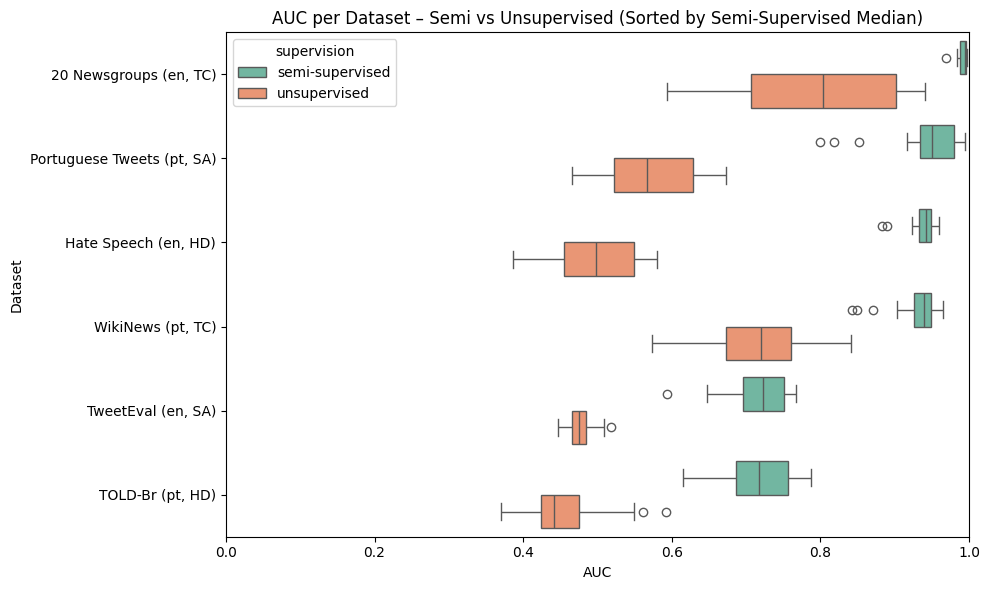
\includegraphics[width=0.85\linewidth]{figs/auc_per_dataset.png}
\caption{AUC per dataset comparing semi-supervised and unsupervised settings. Datasets are annotated with language and task type, and sorted by median AUC in the semi-supervised setting.}
\label{fig:auc_per_dataset}
\end{figure}

This effect is especially evident in semantically complex tasks like sentiment analysis and hate speech detection, where unsupervised models often fail to capture ambiguity, subtle phrasing, irony, or culturally specific hostility. For example, in TweetEval (en) and Portuguese Tweets (pt), distinguishing sentiment nuances is challenging without labels. Similarly, hate speech detection tasks such as TOLD-Br and Hate Speech Tweets benefit greatly from even a small number of labeled examples, which helps models establish clearer decision boundaries.
By contrast, topic classification datasets like 20 Newsgroups (en) and WikiNews (pt) contain more distinct lexical signals—e.g., “graphics” or “politics”—allowing unsupervised models to perform reasonably well. Still, semi-supervised models outperform them, though with smaller gains.

These results challenge the common belief that unsupervised methods suffice due to their generality and low annotation cost. While this may apply to structured data, our findings show that textual anomaly detection benefits substantially from limited supervision, especially in linguistically rich contexts. We also observe cross-lingual differences: English datasets exhibit higher and more stable AUCs, while Portuguese datasets show greater variance and lower baselines—possibly due to label noise, fewer pre-trained encoders, or increased linguistic diversity. The Wilcoxon signed-rank test~\cite{wilcoxon1945individual}, applied to paired AUC scores from multiple model-encoder combinations on each dataset, confirms that the performance improvements with semi-supervised models are statistically significant across all datasets evaluated ($p < 0.001$).

\subsection{RQ2: How does representation type affect performance?}

Figure~\ref{fig:encoder_type_performance} presents the performance distribution of multilingual and Portuguese-specific encoders across the three Portuguese datasets (TOLD-Br, WikiNews, and Portuguese Tweets), analyzed separately under unsupervised and semi-supervised conditions. In the semi-supervised setting, both encoder types achieved competitive AUCs, with models like XLM-RoBERTa (multilingual) and BERT-large-PT (Portuguese-specific) showing relatively stronger results. However, performance variability was evident across encoders, with Serafim, for instance, presenting lower median AUCs compared to the other Portuguese-specific models.
In the unsupervised setting, AUC distributions were broadly dispersed across all encoders, with substantial variability within and across encoder types. Although Portuguese-specific encoders showed slightly higher median AUCs in some cases, the performance distributions of multilingual and Portuguese-specific models largely overlapped.

\begin{figure}[ht]
\centering
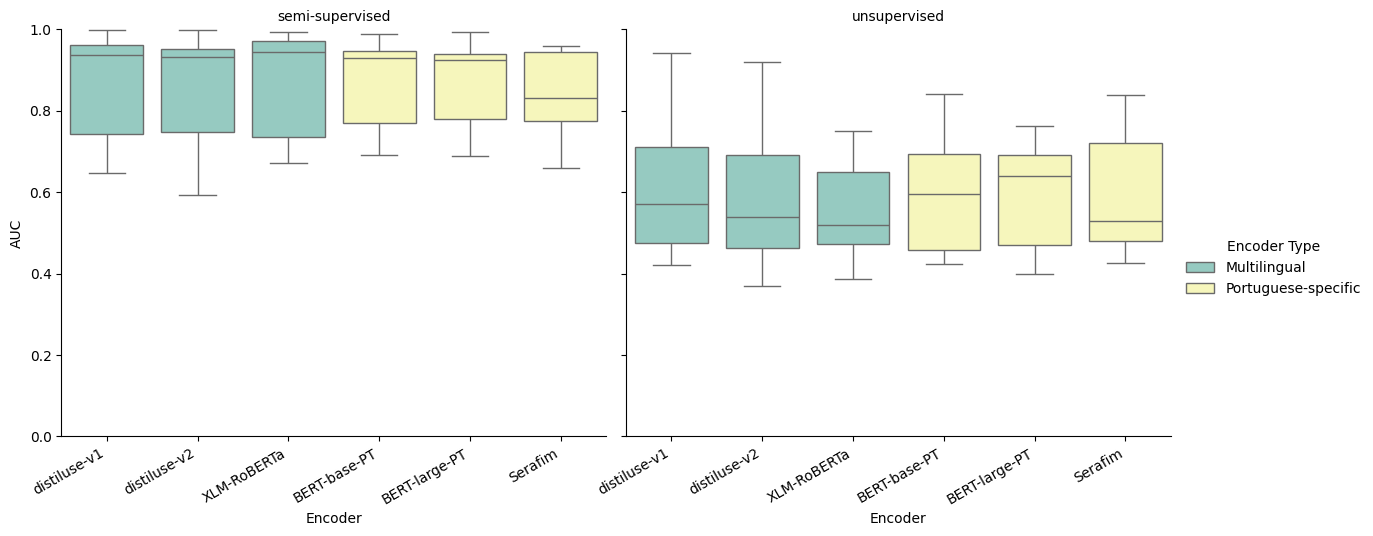
\includegraphics[width=\linewidth]{figs/encoder_type_performance.png}
\vspace{-1em}
\caption{\scriptsize AUC for multilingual and Portuguese-specific encoders under unsupervised and semi-supervised settings (Portuguese datasets only). Encoder names are abbreviated for readability, as listed in Table~\ref{tab:encoders}.}
\label{fig:encoder_type_performance}
%\vspace{-1em}
\end{figure}

To assess whether encoder type influenced anomaly detection performance, we used the Mann–Whitney U test~\cite{mann1947test} to compare AUC distributions between multilingual and Portuguese-specific encoders across the Portuguese datasets. The test indicated no statistically significant difference in either supervision setting (semi-supervised: $p = 0.77$; unsupervised: $p = 0.39$), suggesting that performance variations are more dependent on dataset-specific factors and model configurations than on encoder language scope

\subsection{RQ3: Which Models Are Most Robust Across Tasks and Datasets?}

To evaluate model robustness, we analyze the distribution of AUC scores per model across all datasets and task types under both supervision regimes (Figure~\ref{fig:model_auc_both}). Models such as DevNet and XGBOD consistently deliver strong and stable performance, particularly in semi-supervised settings. Surprisingly, a simple feed-forward MLP also proves competitive, often outperforming more complex unsupervised architectures—highlighting the importance of high-quality representations even in lightweight models.

However, performance varies by task. In topic classification datasets such as \textit{20 Newsgroups} and \textit{WikiNews}, unsupervised methods perform reasonably well. These tasks involve lexical and thematic shifts that align well with density- and distance-based heuristics. In contrast, sentiment analysis and hate speech detection present subtler, context-dependent anomalies that challenge unsupervised models and benefit more from supervision.
In such semantically rich settings, even minimal labeled data enables semi-supervised models to calibrate more discriminative boundaries. This effect is especially apparent in DevNet, XGBOD, and MLP, which frequently exceed 0.90 AUC in semi-supervised mode. These models leverage few-shot signals effectively, suggesting that sparse supervision can dramatically enhance generalization in high-dimensional text spaces. Conversely, models such as DeepSVDD, OCSVM, and LOF show limited effectiveness—particularly in unsupervised configurations. Reconstruction-based methods like AutoEncoder (AE) and Variational AutoEncoder (VAE) achieve intermediate results but generally lag behind their semi-supervised counterparts.

Overall, our findings suggest that model robustness in textual anomaly detection depends on both architectural flexibility and task complexity. The best-performing models pair adaptable learning objectives with strong embeddings, but task semantics remain a critical factor: unsupervised methods are more viable in structured, topical datasets, while semantically nuanced tasks demand supervision to achieve competitive performance.

\begin{figure}[ht]
\centering
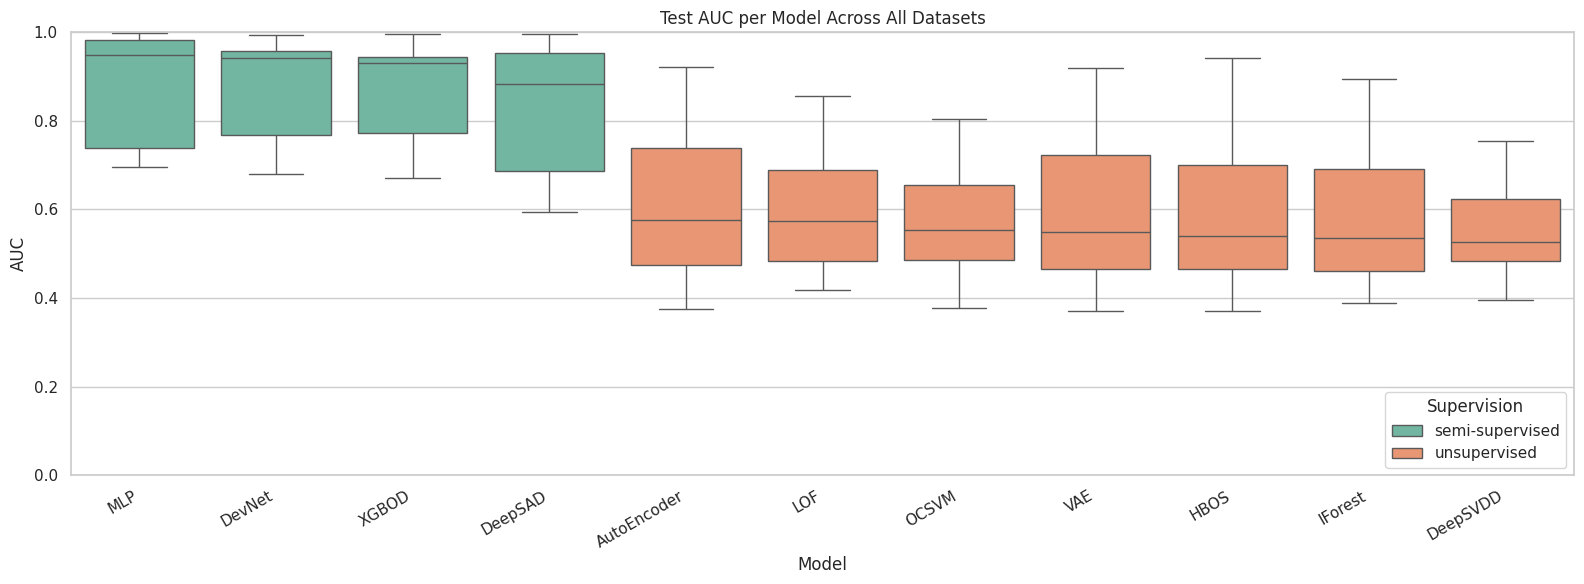
\includegraphics[width=0.9\linewidth]{figs/model_auc_both.png}
\vspace{-1em}
\caption{\scriptsize Test AUC per model across all datasets under unsupervised and semi-supervised settings. Robust models exhibit high median performance and low variance across diverse tasks.}
\label{fig:model_auc_both}
%\vspace{-1em}
\end{figure}
\vspace{-1em}


\subsection{RQ4: How Much Supervision Is Needed to Outperform Unsupervised Methods?}

To assess how much supervision is necessary to surpass unsupervised baselines, we focused on the \texttt{DevNet} model—previously identified as one of the most effective semi-supervised approaches—and applied it across three Portuguese datasets. We progressively increased the number of labeled anomalies, starting from 10 examples and incrementally reaching up to 5\% of the training set. In each round, a small batch of additional anomalies was randomly selected and incorporated into the labeled set. This process was repeated across five random seeds to ensure robustness.

Figure~\ref{fig:degree_of_contamination_random} displays the AUC progression for each dataset as a function of labeled anomaly percentage. Results show that even small amounts of supervision can lead to substantial performance improvements—especially in the early rounds. However, the supervision-efficiency curve varies by task: performance trends differ by task. In \textit{Portuguese Tweets} (sentiment analysis), near-optimal AUC is achieved with less than 1\% labeled anomalies, and variance stabilizes quickly. In \textit{WikiNews} (topic classification), performance improves steadily but saturates earlier and more modestly, suggesting that some tasks generalize well with minimal labels. In contrast, \textit{TOLD-Br} (hate speech detection) exhibits a more gradual and noisy curve, with no clear saturation by 5\%, indicating that semantically complex or ambiguous tasks may require more supervision.

In addition to mean AUC, we observe a clear difference in variance reduction across tasks. For instance, Portuguese Tweets (sentiment analysis) exhibits low variability even with a small number of labels, suggesting consistent patterns are quickly learned. In contrast, TOLD-Br (hate speech detection) shows high variance throughout, underscoring the semantic ambiguity and domain-specific nuances that make the task more label-hungry.
These findings suggest that, in few-shot anomaly detection scenarios, the amount of supervision required to unlock strong performance depends heavily on task complexity. Nevertheless, even randomly selected anomalies are often sufficient to yield meaningful gains, reinforcing the value of lightweight semi-supervised pipelines in practical settings.

\begin{figure}[ht]
\centering
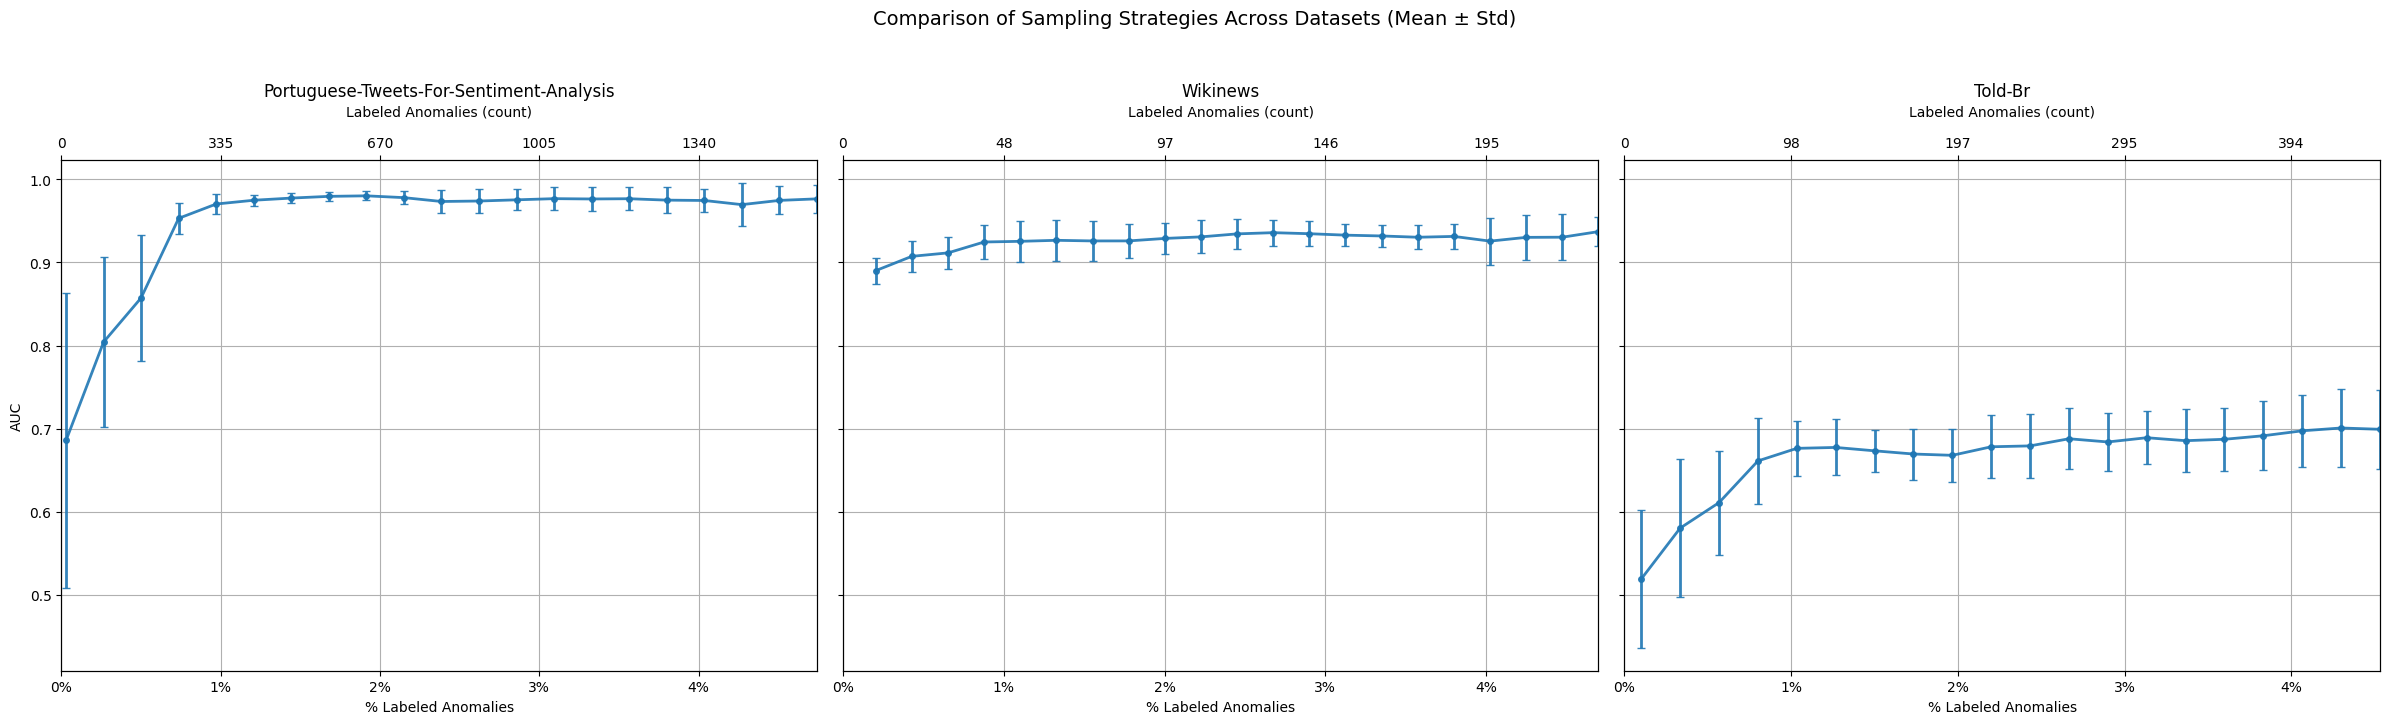
\includegraphics[width=\linewidth]{figs/degree_of_contamination_random.png}
%\vspace{-1em}
\caption{\scriptsize AUC as a function of labeled anomaly proportion (bottom x-axis) and raw count (top x-axis) for three Portuguese datasets using \texttt{DevNet} with random sampling. Each line shows the mean ± standard deviation across five runs. Saturation is reached at different supervision levels depending on task complexity.}
\label{fig:degree_of_contamination_random}
%\vspace{-1em}
\end{figure}
\vspace{-1em}

\section{Conclusion and Future Work}

This study introduced a comprehensive benchmark for anomaly detection in textual data, emphasizing low-supervision scenarios across both Portuguese and English corpora. We compared unsupervised and semi-supervised approaches over six datasets and multiple embedding strategies, including multilingual and language-specific encoders. Our experiments show that even minimal supervision—labeling 1--5\% of anomalies—can yield substantial improvements, especially in semantically complex tasks like sentiment analysis and hate speech detection.

Semi-supervised models such as DevNet, XGBOD, and DeepSAD consistently outperformed unsupervised baselines. Multilingual encoders demonstrated greater robustness when labeled data was scarce, while language-specific models proved highly effective when more labels were available. Importantly, we observed that performance often saturated after only a few annotation rounds, reinforcing the value of few-shot learning for scalable anomaly detection.

Looking ahead, we see several promising directions:
(i) leveraging large language models (LLMs) to generate weak labels, assist with difficult cases, and enable real-time adaptation to new data;
(ii) expanding beyond sentence-level analysis to entities, phrases, and documents to uncover finer-grained anomalies;
(iii) extending this benchmark to additional languages and domains, with particular attention to low-resource settings where labeled anomalies are rare but domain knowledge is crucial; and
(iv) exploring how different representation learning objectives—such as contrastive or attention-based pretraining—affect anomaly detection quality.

\section*{Acknowledgments}
\small
This study was financed in part by the Coordenação de Aperfeiçoamento de Pessoal de Nível Superior – Brasil (CAPES) – Finance Code 001. 
The authors would like to thank the National Council for Scientific and Technological Development (CNPq, grant \#312360/2023-1).
\normalsize

\bibliographystyle{sbc}
\bibliography{refs}

\clearpage


\end{document}
